\chapter{Data Stream Processing}
\label{chap:data_stream_processing}

With the advent of \emph{Big Data} era, large amount of data are being generated 
by the companies from their infrastructure; from the IoT sensors to the events 
generated by the customers using their online services. The data that 
are generated are by nature \emph{unbounded} and infinite since as long 
as the infrastructure is working, new data will be continuously generated. 

For example, the healthcare industry has also been transitioning to 
adopt the approach of data-drive diagnostics methods~\cite{hospital_diagnosis}. 
This transition is caused by the need to keep up with the increase in the amount 
of physiological data generated by the monitoring sensors attached to the 
patients~\cite{hospital_data_monitoring}. These physiological data are generated 
periodically at regular intervals in a streaming manner. 

As a consequence of the large volume and continuous data generation, there is a need for 
the companies to be able to process these unbounded data streams.
Stream processing engines are equipped to handle such unbounded data and exists in 
the industry today (e.g. Apache Flink~\cite{flink} and 
Apache Spark streaming~\cite{spark_streaming}). Main features of these stream 
processing engines are their ability to 
\renewcommand{\labelenumi}{(\roman{enumi})}
\begin{enumerate*}
    \item scale horizontally, 
    \item process records individually as they arrive, and
    \item process or analyse the data in real time.
\end{enumerate*}

In Chapter~\ref{chap:data_stream_processing}, we will dive into details of 
on the characteristics of data streams, how DSMS handles fault tolerance, and
the general strategy to processing the streaming data. Finally, we will also elaborate on the 
various state-of-the-art frameworks in use by the industries.

\section{Characteristics of Data Streams}
\label{sec:characteristics_data_stream}
What is a data stream? As defined by Golab and Ozsu~\cite{golab_data_stream}:
“A \emph{data stream} is a \emph{real-time}, continuous, ordered (implicitly by arrival time 
or explicitly by timestamp) sequence of items. It is impossible to control the order
in which items arrive, nor is it feasible to \emph{locally store} a stream in its entirety.”
The difference between traditional Big Data processing and data stream processing, lies in 
the inability to store the whole dataset \emph{locally} for data streams management. Furthermore, 
data streams processing requires real-time response in most use cases. Therefore, there is a 
difference in the importance of the characteristics from the ones used to define Big Data. 

Big Data is usually characterized with the three “V's: \emph{volume}, \emph{velocity} 
and \emph{variety}~\cite{big_data_analytics}. 
In the context of data streams processing, it is expected that the \emph{volume} of 
the data is unbounded since the devices, sensors and applications are constantly 
generating data as long as there is an uptime. The \emph{variety} aspect of the 
data streams is also heterogeneous in nature where different sources used by the same 
processing engine may emit different types of data; structured and unstructured. 
Moreover, \emph{variety} in data can also happen over time; a concept drift where 
the properties of data may change over time unlike Big Data. 

Out of the three aforementioned characteristics, \emph{velocity} is the most important 
factor to consider when it comes to data stream processing. Data in a streaming 
environment is fast changing, and they arrive constantly into the stream processing
pipeline and needs to be processed in real-time. As a result of the need for real-time 
response, it is infeasible to have random memory access capability --- only single pass algorithm can
be applied. This requirement of low latency processing has a consequence 
that late decisions will result in missed opportunities. Related to \emph{velocity}, 
the data streams can also have a sudden \emph{'burst'} in the arrival rate which varies 
over time. 

In monitoring application of stream processing, the interest lies in the analysis of 
most recent data. As a result, the order of the data sequence needs to be considered 
when processing data streams. Due to the nature of data stream having to be transmitted over a 
network, the ordering of the data cannot be guaranteed. This is 
likely to happen if the network transmission protocols have no guarantee in the global 
ordering of data or if there is latency~\cite{requirements_dsp}. 

In certain applications such as fraud detection in bank transactions and monitoring of 
patient's biometrics, the data streams emitted by the sensors need to be processed in 
real-time. This is because the data streams in such scenarios will rapidly degrade in 
value if they are not handled immediately. Thus, real-time processing of data streams 
is a necessary requirement for data stream processing engines. 

In the context of this work, where the focus is on the application of multi-stream operators, 
the \emph{velocity} of a data stream will have a huge impact on the quality and efficiency of 
the generated results. As a consequence of the challenges brought forth by the 
aforementioned characteristics of data streams, a Data Stream Management System (DSMS) needs 
to be able to deal with them appropriately.  

\section{Data Stream Management Systems (DSMS)} 
Data Stream Management Systems are designed to overcome the aforementioned challenges 
in data stream processing. Different from the common big data processing, DSMS has to be 
able to respond in real-time and process the incoming data with low latency~\cite{data_stream_management}. 
For the former requirement, continuous queries are evaluated repeatedly by the DSMS to react 
to the incoming data. The latter could be tackled by reducing the inter-operator communications 
through optimizing operator scheduling and buffers to reduce network traffic~\cite{low_latency_data_stream}. 



\subsection{Fault tolerance}
As stated in the beginning of this Chapter, DSMS will also have to be able to scale 
horizontally --- stream processing must be distributable over multiple computing nodes. 
This leads to the requirement that there needs to be some form of coordination and fault tolerance 
for distributed processing. The exact details of guarantee fault tolerance differs from 
one framework to the other, however there are general strategies to provide some 
form of fault tolerance according to Gradvohl et al~\cite{fault_tolerance_dsms}.
In the context of this paper, \textbf{fault tolerance} is a crucial requirement when applying
non-trivial operators that are stateful. 
An example for a non-trivial operator would be a recommender algorithm, where 
a user's parameters would need to be kept in state to update them with each new 
interaction event. 
The following sections will describe the commonly used strategies to provide fault tolerance 
in DSMS. 

\subsubsection{Replication of components}
Just as the name suggests, it involves duplicating the components of the stream processing
engine to minimize the error in case of node failures. There are two kinds of replication; 
\emph{active replication} and \emph{passive replication}. In \textbf{active replication,}
duplicated components are executed just like normal components and receives the same incoming data. 
Therefore, there are duplicates in the output --- this allows the engine to check the 
output to identify errors in the normal components. The disadvantage of this method is 
the increase in the cost due to component duplication. 

\textbf{Passive replication} has inactive duplicated components instead. These backup
components are then on standby to replace their counterpart if there is a failure. This 
reduces the performance cost of executing the duplicated components at the same 
time as their counterpart. However, starting the backup component requires the input 
to be resubmitted for it to catch up and return to normal state. This results in a significant 
delay every time there is a failure and not acceptable for the requirement of real-time response. 


\subsubsection{Checkpoint}

Checkpoints represent states the DSMS could be in at a certain point in 
time in each of the input streams along with the corresponding 
state for each operator. Snapshots of records for each checkpoint are also kept 
by DSMS to be replayed in case of failure. 
In this fault tolerance strategy, a DSMS is modelled by a sequence of 
checkpoints which are fault free~\cite{fault_tolerance_dsms}. 

In the case of a failure, the operators will be restarted and set back to the state of the 
last successful checkpoint. The records, which were part of the failure, will be replayed
at the input using the snapshot of the state. 

There are two approaches to implement checkpoint at the operator-level; 
\emph{asynchronous} and \emph{synchronous} checkpoints~\cite{fault_tolerance_dsms}.

Uncoordinated checkpoints do not guarantee a global state consistency, since 
each operator performs a checkpoint on their state independently. This results 
in less overhead of saving the state of the whole system with the disadvantage of the higher 
difficulty to recover back to a consistent global state. Figure~\ref{fig:checkpoint_inconsistency}
shows a scenario where uncoordinated checkpoint strategy results in inconsistency of 
global state. In this example, message \emph{m} is not part of the checkpoint of operator 
A even though operator B includes the sending of ~\emph{m} as part of its checkpoint. Therefore, 
rolling back to this checkpoint will result in an inconsistent global state, causing the 
DSMS to rollback to an earlier consistent checkpoint. At worst case, this could result 
in the DSMS trying to repeatedly rollback until a consistent checkpoint is met, 
resulting in a 'domino effect'.  

On the other hand, in coordinated checkpointing, the operators will take a snapshot 
of their internal state at the same "time" and save them to provide a consistent 
global state, avoiding the 'domino effect' of asynchronous checkpointing. To ensure 
the global consistency, a global synchronization mechanism is required. A simple 
algorithm to achieve this mechanism, is to have a central coordinator to synchronize 
the checkpointing process amongst the different operators. This brings with it an overhead 
of coordinating these operators, increasing the latency of the operators whenever a 
checkpoint has to be taken. 


There exists algorithm which combines the best of both world; asynchronous, non-blocking
operators for checkpointing with the consistency of global states. 
Chandy-Lamport algorithm~\cite{chandy_lamport} is one such algorithm to determine the 
global states of a distributed system which could be used to maintain the checkpoints. 

\begin{figure}[!htbp]
    \centering
    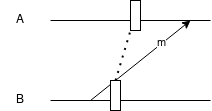
\includegraphics{fig/checkpoint_inconsistency.png}
    \label{fig:checkpoint_inconsistency}
    \caption{Operator B sends a message \emph{m} to operator A and both operators 
    committed a checkpoint of their internal state.}
\end{figure}

\subsubsection{Upstream backup}

\begin{figure}[!htbp]
    \centering
    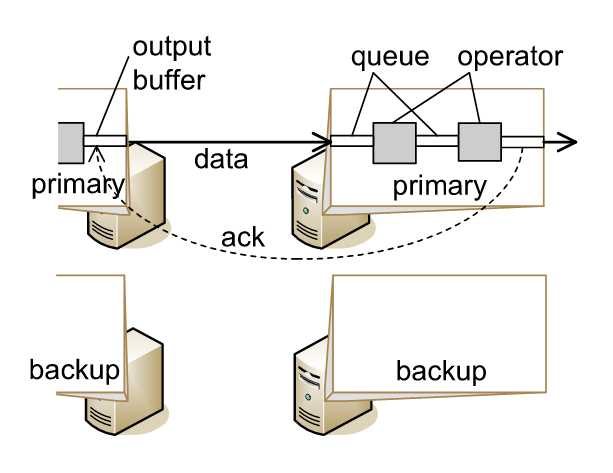
\includegraphics[width=0.5\textwidth]{fig/upstream.png}
    \label{fig:upstream}
    \caption{Upstream backup~\cite{upstream_backup}. }
    
\end{figure}


In this approach of fault tolerance, up stream nodes will temporarily 
keep the tuples in their output buffer for the subsequent nodes. The tuples 
stay in the buffer until they are completely processed by the child node. 
The buffer will then be cleared when the parent node receives 
an acknowledgement from its children, as illustrated in Figure~\ref{fig:upstream}. 

The drawback for this approach is that, the buffer might not be large enough to 
hold the tuples stored between the failure and the recovery event. Moreover, 
the whole system needs to be halted until the new node catches back up to 
the state of the failed node from the replayed tuples. 

\subsection{Data processing}

Owing to the characteristics described in Section~\ref{sec:characteristics_data_stream}, 
processing data streams requires a different approach from a typical data processing engine. 




